\documentclass[11pt,a4paper]{article}
\usepackage[T1]{fontenc}
\usepackage[utf8]{inputenc}
\usepackage{lmodern}
\usepackage[margin=28mm]{geometry}
\usepackage{amsmath,amssymb,amsthm,mathtools}
\usepackage{booktabs,array,tabularx}
\usepackage{graphicx,tikz}
\usetikzlibrary{arrows.meta}
\usepackage[section]{placeins}
\usepackage{float}
\usepackage[skins]{tcolorbox}
\newtcolorbox[auto counter,number within=section]{formalnote}[1]{
 enhanced,colback=black!2,colframe=black!40,
 colbacktitle=black!7,coltitle=black,boxrule=.4pt,arc=1pt,
 left=9pt,right=9pt,top=7pt,bottom=7pt,
 fonttitle=\bfseries,fontupper=\small,
 title={Formal \thetcbcounter: #1},before skip=12pt,after skip=12pt
}
\usepackage{microtype}
\usepackage[authoryear,round]{natbib}
\usepackage[hidelinks]{hyperref}
\usepackage{bookmark}
\hypersetup{pdftitle={A Geometrical Theory of Communication: Measurement, Meaning and Representation},
 pdfauthor={Walter Henrique Alves da Silva},
 pdfsubject={Geometric bit, measurement, identity and representation}}
\setlength{\emergencystretch}{2em}
\newtheorem{theorem}{Theorem}
\newtheorem{proposition}[theorem]{Proposition}
\newtheorem{corollary}[theorem]{Corollary}
\theoremstyle{definition}
\newtheorem{definition}{Definition}
\newcommand{\R}{\mathbb R}
\newcommand{\C}{\mathbb C}
\newcommand{\Z}{\mathbb Z}
\newcommand{\HH}{\mathbb H}
\newcommand{\E}{\mathbb E}
\newcommand{\Prob}{\mathbb P}
\newcommand{\id}{\mathrm{id}}
\newcommand{\SO}{\mathrm{SO}}
\newcommand{\SU}{\mathrm{SU}}
\newcommand{\dist}{\mathrm d}
\DeclareMathOperator{\Rea}{Re}
\DeclareMathOperator{\Ima}{Im}
\DeclareMathOperator{\diam}{diam}
\title{A Geometrical Theory of Communication:\\
Measurement, Meaning and Representation}
\author{Walter Henrique Alves da Silva\\\small Independent researcher\\
\small ORCID: \href{https://orcid.org/0009-0001-0857-096X}{0009-0001-0857-096X}}
\date{Version 1 --- working draft --- 23 September 2026}
\begin{document}
\maketitle

\begin{abstract}
What makes an alternative identifiable before we count it? Shannon's
information measure begins with distinguishable possibilities and
assigns an amount to the uncertainty of their selection. I trace
that measurement back to the comparison it uses: a held reference,
distinct readings, and a unit that remains the same when repeated.
The geometric bit brings these relationships together through the
circle, where perpendicularity, symmetry, and closure give identity
an operational form. Euler's formula expresses their composition.
The argument places this geometric identity at the foundation of
counting and communication, then follows three questions: what
exists, what do we measure/observe, and how do we convey it?
Physical interaction, measurement, division algebras, Hopf projections,
and language enter as parts of the account of how an identity
becomes available, survives a change of expression, and is recovered
by another observer.
\end{abstract}

\section*{Introduction}
\label{sec:opening}

\emph{What is information? What does that mean?}

Ask anyone and you get an answer, quickly: news, data. knowledge, bits,
something I did not know before. Everyone reaches for it, everyone
reaches somewhere a bit different but the word keeps working, as it has been
doing so for a long time: \emph{informare}, to give form, to shape, to
inform someone is to give a shape to what they know. Shannon gave us a precise
answer in \emph{A Mathematical Theory of Communication}: a measure of
uncertainty, defined through entropy, that set the quantitative
foundation of information theory and modern communication
\citep{Shannon1948}. But uncertainty about what? Does that answer our question about what information is? Bear with me as we unpack this question thoroughly.

Asking what information is already assumes that the question has an
object---that the word points to something, whether we call it data or
knowledge, it's an object that exists in some sense, even if abstract. Let us say it does, and let us say that I, the author, have
seen it and measured it, and so I know what information is. How do I
transfer that knowledge to you, the reader? How do I give you
information about information? And how do you know that knowledge is true?

Weaver already wrote down the three levels of communication problems
\citep[pp.~4--5]{ShannonWeaver1949}. Word for word:
\begin{description}
  \item[Level A --- Transmission.] How accurately can the symbols of
  communication be transmitted? (The technical problem)
  \item[Level B --- Meaning.] ``How precisely do the transmitted symbols
  convey the desired meaning?'' (The semantics problem)
  \item[Level C --- Effectiveness.] ``How effectively does the received
  meaning affect conduct in the desired way?'' (The effectiveness problem)
\end{description}
The original mathematical theory solved Level A, and Shannon drew that
boundary himself: the semantic aspects of communication ``are irrelevant
to the engineering problem'' \citep[p.~379]{Shannon1948}. He was right about the engineering: the mathematics works, and a great deal of current technology runs on it. Information came away from that work with a number attached, our computational bit, while most of our questions about what information actually is remain open. The level B problem is exactly what this paper is going after.

Let's say I point to a lighter on the desk between us: we both see it, and we both
know that it is there. What does that mean? The word \emph{lighter}
points to an object in the world, and our two perspectives on that
object still point the same word at the same thing. I could call it an
igniter and you would receive the same information through a different
symbol, the word carries a meaning we can already both reach.

The physical object, our perspective on it, and the symbol we use to represent it. three questions separate the objects here, and together they answer what information
is. What exists as a physical entity? How do we observe, measure or know it? How do we represent and transfer that knowledge?

This is a unavoidably an interdisciplinary subject: for what counts as existing, we need physics; to know that it holds
independently of my beliefs, we need epistemology; to convey it, we need
linguistics, mathematics and Shannon's original paper---because as soon
as I know it and set out to tell you, we are already inside Level B, how do I give you information about information through my own set, and how can you know it's true?

The first part of this paper works through an object where the
separation between reality, measurement and notation stays visible: a
circle. Closure over rotation, written by Euler as a mathematical
identity, supplies the preserved relationship we need to answer the
question of information in a precise and robust way. Shannon's
definition of the bit aimed at the same target, and his description
returns here as a partial case, pairing entropy with geometric closure.
That yields a definition of a \emph{geometric bit}: a unit of comparison
that retains a distinction together with the reference needed to
interpret it.

If I say A, you must understand A for that meaning to have been communicated.
The agreement between \emph{igniter} and \emph{lighter} already depends
on this: the expressions differ, while what they mean in that encounter
is the same. Language allows variation in how much is understood, but
communication requires this shared ground; scientific descriptions depend
on agreement precise enough to identify the same subject and follow the
same claim; and for mathematical objects, their defining relationships make
that requirement exact ---an identity.

Defining the geometric bit gives the principle of identity, $A=A$, an
operational form: the identity required for meaning to pass from one
person to another is built into the unit itself. This connects the two
parts of the paper: establishing what information is establishes the
identity to be conveyed, and the theory of its transmission asks how
that identity is preserved between sender and receiver.

The second part asks how to send it, now with the unit in hand: what must a description
retain for a reader to recover the comparison it was about, how do
several comparisons combine, and how much of one survives noise and
limited precision?

\subsection*{A note on interdisciplinarity}

Where should an account of information begin if its meaning depends on
all three questions? A record has a physical realization, as Landauer
emphasizes \citep{Landauer1996}, and obtaining a reading requires an
interaction with what is being observed. Quantum information makes this
connection especially clear by relating what can be distinguished to
the states and measurements a physical system allows
\citep{NielsenChuang2010}. Physics enters the inquiry wherever a claim
about information depends on how a distinction is made in the world.

Expressing that distinction mathematically makes its relationships
precise enough to calculate and compare. Computing and machine learning
ask how representations can be used and learned; psychology asks how
people learn to recognize what a sign means; philosophy and epistemology
ask what grounds that recognition as knowledge. These concerns meet in
Level B, where checking whether meaning was conveyed requires both an
account of what was meant and a way of recognizing its recovery.

The same problem applies to the paper itself: its symbols are meant to
convey relationships that a reader can understand and check. Information
theory has a metascientific role in this sense, since every science
records observations and communicates what is known through descriptions.
The interdisciplinary approach follows those connections, from what
exists, through how it becomes known, to how that knowledge becomes
available to someone else.

\section{From Shannon's bit to the geometric bit}
\label{sec:v1-comparison}

How did Shannon and Weaver make the transmission problem measurable?
They set meaning aside on purpose: a message full of meaning and a
string of nonsense can have the same information measure, because
the task is to recover at one end the message selected at the other.
The uncertainty concerns which of the possible messages was chosen,
so the measure belongs to the whole choice situation
\citep[pp.~8--9]{ShannonWeaver1949}.

\subsection{Shannon's bit: what the choice already assumes}

Weaver's example makes this easy to see. The two possible messages
are the whole King James Bible and the single word ``Yes.'' One is
a book and the other is a word, yet either can be selected by the
same small signal: we agree beforehand that $0$ selects the Bible
and $1$ selects ``Yes,'' or that a closed relay selects one and an
open relay the other. I already have the messages and their labels;
when your signal arrives, I learn which one you chose.

With the alternatives equally likely, we assign this choice the
value one and call its unit a bit, John Tukey's contraction of
\emph{binary digit}. Weaver calls the assignment a convention:
the unit measures the choice between the two messages, whatever
their length or meaning \citep[p.~9]{ShannonWeaver1949}.

What happens when we have more choices? Two independent binary
choices give four possible pairs, and three give eight possible
triples. The possibilities multiply while the information adds,
which is the counting rule expressed by the logarithm. Unequal
probabilities change how much we learn: an almost certain answer
is less surprising than a rare one, and entropy averages over
these possibilities \citep{Shannon1948}.

\begin{formalnote}{The choice, its unit, and entropy}
For a finite set of $N$ equally likely messages, the information is
$I(N)=\log_2N$, with $I(2)=1$ fixing the unit. Independent choices
multiply the number of possibilities, so
\[
 I(NM)=I(N)+I(M).
\]
The logarithmic form follows from additivity and regularity. For
a continuous extension $J$ to positive arguments satisfying
$J(xy)=J(x)+J(y)$, the function $g(t)=J(e^t)$ is continuous and
additive, hence $g(t)=ct$. Thus $J(x)=c\ln x$, and $J(2)=1$
gives $c=1/\ln2$.

For a message $m$ of probability $p(m)>0$, its self-information is
$-\log_2p(m)$. The source entropy is its expectation,
\[
 H(M)=-\sum_m p(m)\log_2p(m),\qquad 0\log_2 0:=0.
\]
A binary source has $0\leq H(M)\leq1$, with equality at the upper
bound precisely for equal probabilities. Two available states and
one bit of entropy coincide in that case \citep{Shannon1948}.
\end{formalnote}

How does the bit look geometrically? Put $0$ and $1$ on a line,
holding $0$ as the reference and placing $1$ one unit away. Reading
the mark means comparing its position with that origin and unit.
If we move along the line, the reading changes; if we move along
the perpendicular through $1$, it stays at $1$, just as a ruler's
tick carries a reading across the page.

\begin{figure}[H]
\centering
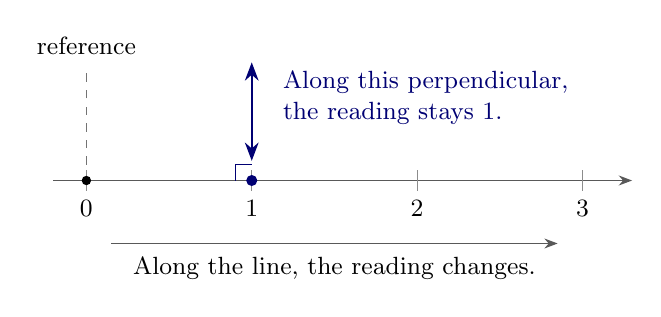
\begin{tikzpicture}[x=2.1cm,y=1cm,>=Stealth,font=\small]
\draw[black!65,->] (-.2,0)--(3.3,0);
\foreach \x in {0,1,2,3} {
  \draw[black!45] (\x,-.13)--(\x,.13);
  \node[below] at (\x,-.13) {$\x$};
}
\draw[black!55,dashed] (0,.2)--(0,1.45);
\draw[blue!45!black,thick,<->] (1,.25)--(1,1.5);
\draw[blue!45!black] (.90,0)--(.90,.2)--(1,.2);
\fill (0,0) circle (1.7pt);
\fill[blue!45!black] (1,0) circle (2pt);
\node[anchor=west,align=left,blue!45!black] at (1.13,1.05)
  {Along this perpendicular,\\the reading stays $1$.};
\draw[black!65,->] (.15,-.8)--(2.85,-.8);
\node[below] at (1.5,-.85) {Along the line, the reading changes.};
\node[above,align=center] at (0,1.48) {reference};
\end{tikzpicture}

\caption{A reading and its reference. Movement along the horizontal
line changes the reading; movement along the perpendicular through
$1$ preserves it. The interval from $0$ to $1$ fixes the unit.}
\label{fig:v1-reference}
\end{figure}

Extend the line to $2$ and $3$, and the same comparison repeats:
the interval from $1$ to $2$ must agree with the interval from $0$
to $1$. Translation carries one interval onto the next while
preserving its length. In this physical account of counting,
perpendicularity keeps the coordinate readings separate and
symmetry keeps the repeated step the same, whether or not we
draw every tick.

\begin{formalnote}{What the perpendicular preserves}
Fix a Euclidean plane, an origin $o$, a unit direction $u$, and a
length unit $\ell>0$. The reading of a point $p$ along that direction is
\[
 x(p)=\frac{\langle p-o,u\rangle}{\ell}.
\]
A displacement $v$ preserves the reading exactly when
\[
 x(p+v)-x(p)=\frac{\langle v,u\rangle}{\ell}=0,
 \quad\text{that is, }v\perp u.
\]
Thus each fixed reading is a line perpendicular to $u$. The points
$p_k=o+k\ell u$ have readings $k$, and translation by $\ell u$
sends $p_k$ to $p_{k+1}$ while preserving distances. These are the
projection and equal-step properties used by the ruler construction.
\end{formalnote}

What happens when we put two bits together? Each must be able to
change while the other stays fixed, giving the four readings
$00$, $01$, $10$, and $11$ at the corners of a square. A third bit
adds another perpendicular coordinate and gives the eight corners
of a cube; each further bit adds another direction in which the
record can vary. An $n$-bit string is one corner of this cube,
read from the common starting corner $00\ldots0$
\citep[Chapter~1]{ODonnell2014}.

\begin{figure}[H]
\centering
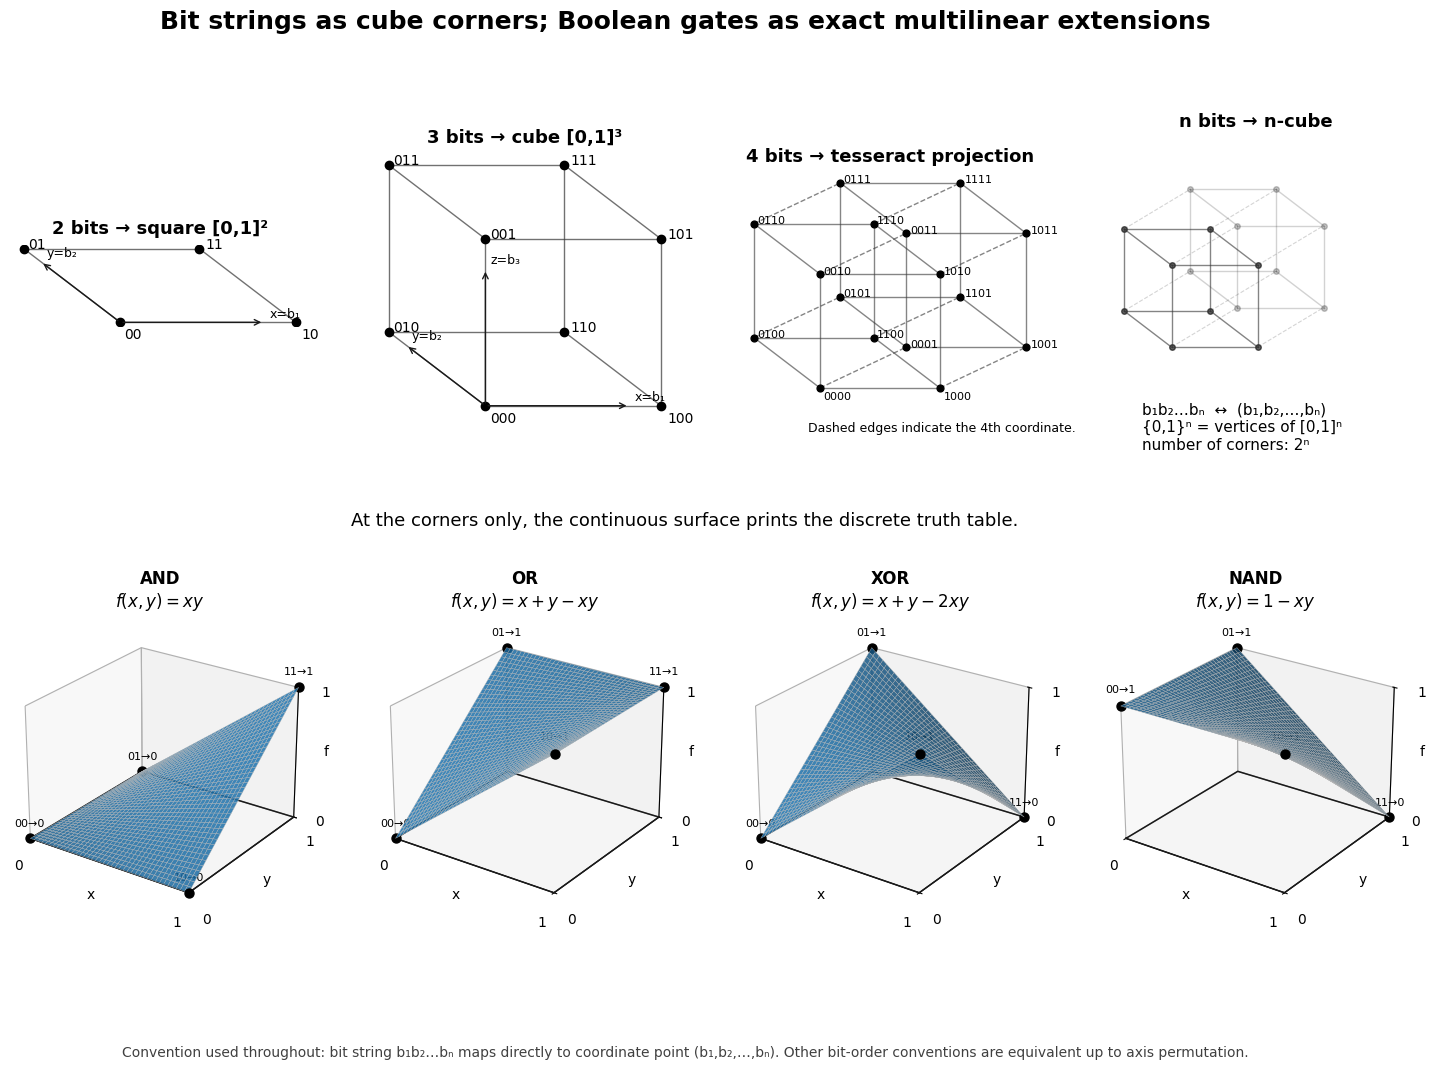
\includegraphics[width=\textwidth]{figures/binary-cube-gates.png}
\caption{Binary states and their operations read geometrically. The
upper row follows independently variable bits into squares, cubes,
and higher-dimensional cubes. Below, each surface gives a gate's
output at its input corners. The surfaces are the corresponding
multilinear extensions of the truth tables.}
\label{fig:v1-binary}
\end{figure}

Computers already use this geometry in their operations. On the
square in Figure~\ref{fig:v1-binary}, AND returns one only at $11$,
just as multiplication $xy$ does. XOR returns one at $01$ and $10$,
where the inputs differ, and zero where they agree. Each gate reads
a corner and supplies an output that another gate can use, allowing
these small comparisons to combine into a computation.

\begin{formalnote}{Gates as functions on the cube}
The binary state space is $B_n=\{0,1\}^n\subset\R^n$, with
$2^n$ vertices and one coordinate per bit. A Boolean gate
$f:B_n\to\{0,1\}$ has the unique multilinear extension
\[
 F(x)=\sum_{a\in B_n}f(a)
       \prod_{j:a_j=1}x_j\prod_{j:a_j=0}(1-x_j).
\]
At a vertex $b$, the product indexed by $a=b$ is one and all others
vanish, so $F(b)=f(b)$. These products form a basis for the
multilinear polynomials, establishing uniqueness within that class.
For two inputs,
\[
 F_{\mathrm{AND}}(x,y)=xy,\qquad
 F_{\mathrm{XOR}}(x,y)=x+y-2xy.
\]
The surfaces in the figure are these extensions; the gate's binary
outputs are their values at the corners
\citep[Section~1.2]{ODonnell2014}.
\end{formalnote}

The cube also tells us how far apart two messages are. A flipped
bit moves a record along one edge, so the shortest route between
two corners counts the positions where their strings differ.
That count is Hamming distance, and zero means the same string.
To correct errors, choose valid records far enough apart that a
few wrong bits still leave the received corner closest to the one
that was sent \citep{Hamming1950}.

\begin{formalnote}{Distance and recovery}
For $x,y\in B_n$,
\[
 d_H(x,y)=\sum_{j=1}^n\mathbf{1}_{x_j\ne y_j}
         =\sum_{j=1}^n(x_j-y_j)^2
         =\|x-y\|_2^2.
\]
Each summand is zero or one. This is also the shortest edge-path
length on the cube: each differing coordinate must be flipped at
least once, and flipping each once reaches the destination.

For a code $C\subseteq B_n$ with at least two codewords, let
$d_{\min}=\min_{c\ne c'\in C}d_H(c,c')$. If $d_{\min}\geq2t+1$,
nearest-codeword decoding corrects any pattern of at most $t$ bit
errors. A word within $t$ of two codewords would, by the triangle
inequality, put them at distance at most
$2t$, contradicting the separation \citep{Hamming1950}.
\end{formalnote}

Some computers even used the cube to connect their hardware.
The Connection Machine CM-1 linked 4,096 routing nodes in a
12-dimensional Boolean cube, with neighbouring addresses differing
in one bit. Moving a message between nodes followed the same
coordinate changes used to compare their addresses
\citep[Section~4.3]{Hillis1985}.

What, then, has the bit given us? A difference recorded against a
fixed reference, a way to combine such records, and operations for
computing with them and recovering them after noise. The agreement
about what each record selects remains in place throughout. If you
send $0$ for the Bible while I read $0$ as ``Yes,'' the string arrives
correctly and I still recover the wrong message.

\begin{formalnote}{The shared agreement}
For the agreed repertoire $\mathcal M=\{\text{Bible},\text{Yes}\}$,
let the sender's encoding be $E_S:\mathcal M\to\{0,1\}$, with
$E_S(\text{Bible})=0$ and $E_S(\text{Yes})=1$. Let
$D_R:\{0,1\}\to\mathcal M$ be the receiver's interpretation.
If $b=E_S(m)$ is sent and $\hat b$ is recovered, the two checks are
\[
 \hat b=b,\qquad D_R(\hat b)=m.
\]
With exact symbol recovery, agreement for every message requires
$D_R\circ E_S=\mathrm{id}_{\mathcal M}$. This equation specifies
recovery within the agreed repertoire; the assignment of labels
to its members is part of the setup. Reversing $D_R$ preserves
symbol recovery while making the second check fail.
\end{formalnote}

Every transmitted record therefore leaves us with two questions:
did the receiver recognize the state that was sent, and did that
state select the same thing for both of us? The first is Shannon's
technical problem; the second is Weaver's Level B
\citep[pp.~4--5]{ShannonWeaver1949}. How can that agreement become
something we perform and check, instead of something we assume
when assigning the labels?

\subsection{The geometric bit: identity through an operation}

Draw a circle and mark a starting point. Its boundary separates
inside from outside, and following it brings us back to the mark
after a full turn. We can watch the position change throughout
the movement and compare the result with the reference from which
we began.

Imagine the circle as a pizza to be divided into four equal pieces.
Do we need a compass to recognize where the cuts should go? A
diameter and its perpendicular give four right-angle sectors, a
relationship we can see before drawing the lines. Their opposite
ends give four poles, and turning the arrangement keeps the cuts
at right angles and the poles opposite.

\begin{figure}[H]
\centering
\resizebox{.85\textwidth}{!}{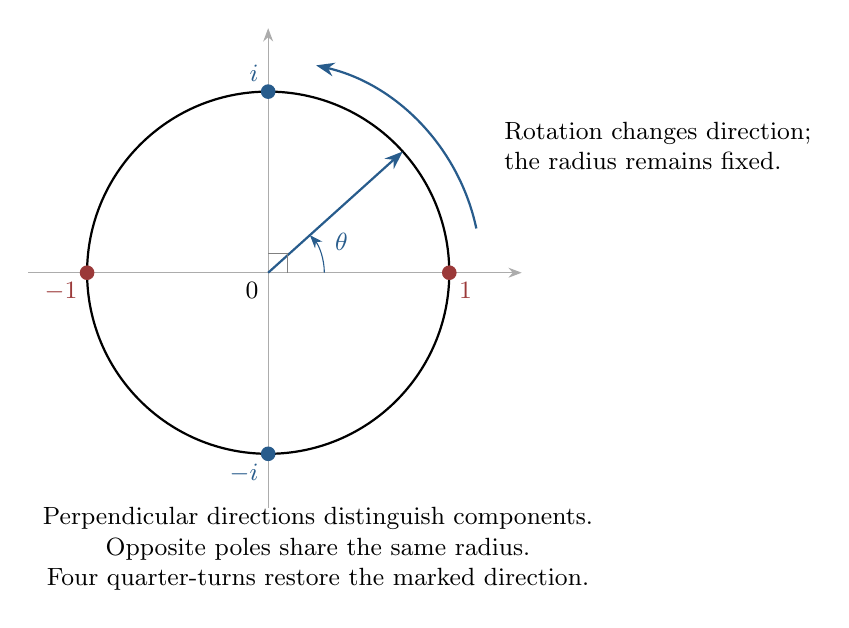
\begin{tikzpicture}[>=Stealth,scale=1.15,every node/.style={font=\small}]
  \definecolor{comparisonblue}{RGB}{40,92,140}
  \definecolor{comparisonred}{RGB}{155,57,57}
  \draw[gray!65,->] (-2.65,0)--(2.8,0);
  \draw[gray!65,->] (0,-2.6)--(0,2.7);
  \draw[thick] (0,0) circle (2);
  \draw[comparisonblue,thick,->] (0,0)--(42:2);
  \draw[comparisonblue,->] (.62,0) arc (0:42:.62);
  \node[comparisonblue] at (23:.88) {$\theta$};
  \draw[comparisonblue,->,thick] (12:2.35) arc (12:77:2.35);
  \node[align=left,anchor=west] at (2.5,1.4)
    {Rotation changes direction;\\the radius remains fixed.};
  \draw[gray] (.21,0)--(.21,.21)--(0,.21);
  \fill[comparisonred] (2,0) circle (2.3pt);
  \fill[comparisonred] (-2,0) circle (2.3pt);
  \fill[comparisonblue] (0,2) circle (2.3pt);
  \fill[comparisonblue] (0,-2) circle (2.3pt);
  \node[comparisonred,below right] at (2,0) {$1$};
  \node[comparisonred,below left] at (-2,0) {$-1$};
  \node[comparisonblue,above left] at (0,2) {$i$};
  \node[comparisonblue,below left] at (0,-2) {$-i$};
  \node[below left] at (0,0) {$0$};
  \node[align=center] at (.55,-3.05)
    {Perpendicular directions distinguish components.\\
     Opposite poles share the same radius.\\
     Four quarter-turns restore the marked direction.};
\end{tikzpicture}
}
\caption{One construction joins distinction and preservation. The
perpendicular axes separate component directions; each axis has
opposite poles; rotation changes their orientation together while
preserving their lengths and angles. A mark distinguishes the
positions through which the circle can be traversed.}
\label{fig:v1-circle}
\end{figure}

Take a reading, turn the arrangement, and compare it with the first.
The marks have moved, while the radius and right angles remain.
We can check whether the drawing has rotated or been distorted by
measuring these lengths and angles. A quarter-turn takes one pole
to its perpendicular, a half-turn takes it to the opposite pole,
and a full turn brings it back to the starting point.

What happens if you begin from a different direction? Put your
reference at the top of the circle while I put mine on the right,
and let us both make a quarter-turn in the same direction. Our
marks finish at different places, but each has turned through the
same angle relative to its own reference. Rotating a reference
and its reading together adds the same angle to both; their
difference stays fixed. We can compare our results because the
reference travels with the reading, and the turn carries its own
direction in the order its positions are reached.

Now change the size of your circle. Its circumference and diameter
grow together, keeping the ratio $\pi$, while the right angles and
the fraction of a turn remain unchanged. We can use different
radii and different starting directions and still check the same
quarter-turn. The shared result is available through the comparison
we perform, rather than through agreement on a particular drawing.

To follow this movement continuously, hold the radius fixed and
let its direction turn. Successive angles add, giving the same
result as the combined turn performed at once. The exponential
expresses this continuous composition; for a pointer turning at
a fixed rate, elapsed time determines how much angle has accumulated.
A complete traversal supplies an event we can record and repeat.

Where is the point now, and how many turns has it made? These are
different readings of the same movement. After each full turn the
point is back at its reference, while the retained count increases
by one. Each repetition uses the same completion criterion, just
as each interval on the numbered line uses the same length.
Addition collects these repetitions, and multiplication collects
equal groups of them.

Let $1$ mark the initial unit radius and multiplication by $i$
perform a positive quarter-turn. Two applications reach the opposite
direction, $-1$, giving $i^2=-1$; the third reaches $-i$, and the
fourth returns to $1$. Euler's formula describes the intermediate
angles, with the half-turn and full-turn values written as
\[
 e^{i\pi}+1=0,\qquad e^{2\pi i}=1.
\]
The first records opposition through cancellation; the second
records the completed return. Starting with any marked radius $A$,
a full turn gives $e^{2\pi i}A=A$: we have an operation through
which the equality can be checked.

I call this repeatable comparison the \emph{geometric bit}.
Shannon's transmission problem takes the identities of the
alternatives and their agreed interpretation as given, then checks
whether the selected symbols are recovered. The geometric bit
makes $A=A$ operational by carrying the reference, the transformation,
and the comparison through which the result is recognized.
This is the account of identity developed here for Level B:
another person can follow the expression and reproduce the
relationship it describes.

For example, you can draw the two perpendicular diameters while
I follow four quarter-turns. We can compare where the poles lie,
the angles between them, and the return to the starting point.
The drawing and the formula direct us to the same checks, allowing
us to establish what we understood through what we can reproduce.

To take a binary reading from the circle, record which side of a
diameter contains the mark, with a convention for points on the
diameter. Using two perpendicular diameters gives four quadrants;
we can retain their labels while setting aside the exact angles.
Once these alternatives and their probabilities are specified,
Shannon's measure applies to the choice among them.

What follows when we compose turns about different spatial axes?
Their order can change the result, so we must keep track of which
turn came first. Quaternions describe this composition while
preserving lengths. The normed division algebras extend the
construction from complex numbers through quaternions to octonions,
retaining the earlier algebra inside the next and preserving the
unit norm under multiplication \citep{Baez2002}.

The associated Hopf maps describe what a projection leaves visible:
several states give the same reading, and the alternatives left
unresolved form its fibre. In this family, the total space at one
level reappears as the fibre type at the next. Section~\ref{sec:v1-physical}
follows this construction beyond the circle on the page into
spatial orientation and its changing views.

Figure~\ref{fig:v1-two-bits} brings the two descriptions together.
We began with a signal whose alternatives and interpretation were
already available, then followed the counting back to a unit we
could repeat and check. To ground that comparison and carry it
between observers, we return to the questions from the introduction:
what exists, what do we measure/observe, and how do we convey it?

\begin{figure}[p]
\centering
% Vector comparison plate. Coordinates are centimetres; no raster assets.
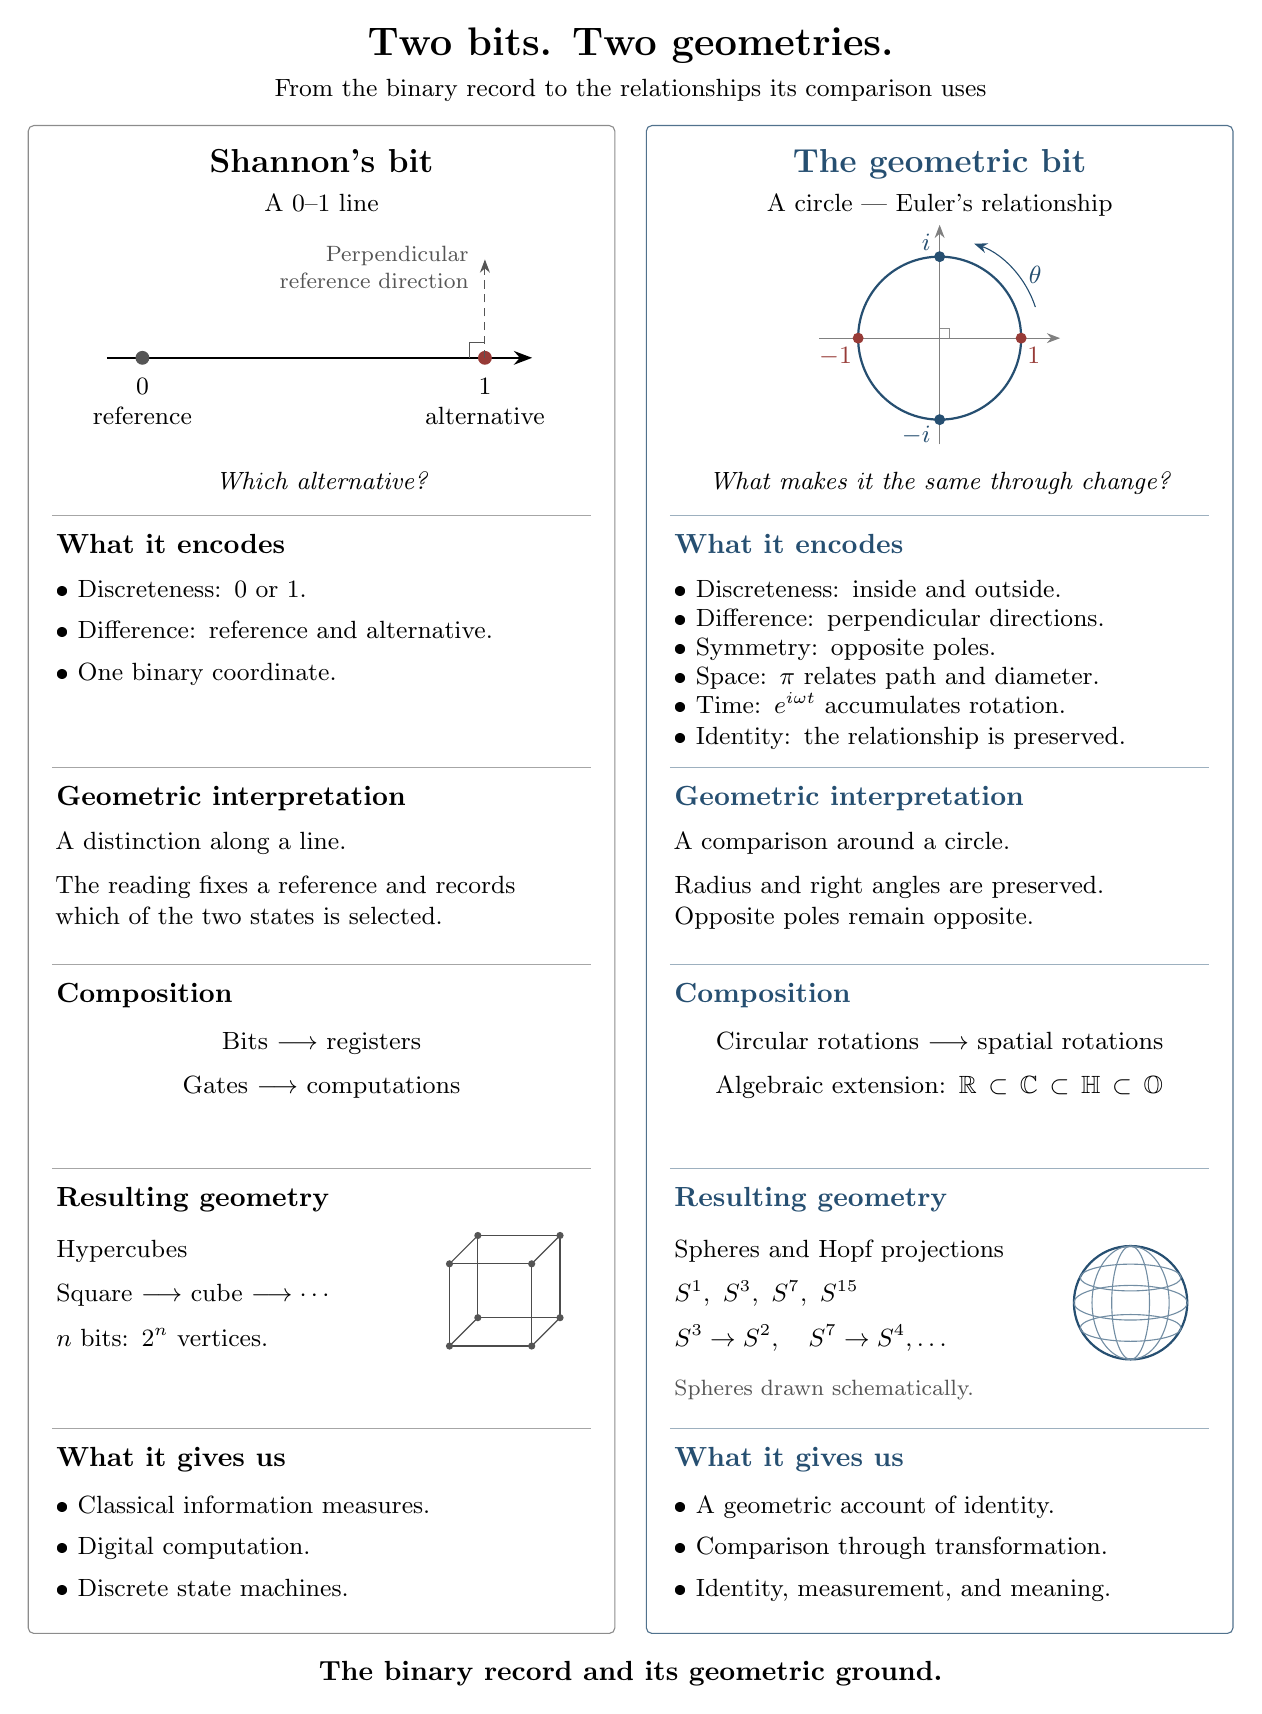
\begin{tikzpicture}[x=1cm,y=1cm,>=Stealth,
  every node/.style={font=\small,inner sep=0pt}]
\definecolor{bitblue}{RGB}{38,79,113}
\definecolor{bitred}{RGB}{151,59,55}
\definecolor{bitgray}{RGB}{85,85,85}

\node[font=\Large\bfseries,anchor=north] at (7.65,0)
  {Two bits. Two geometries.};
\node[font=\small,anchor=north] at (7.65,-.65)
  {From the binary record to the relationships its comparison uses};

\draw[black!45,rounded corners=2pt] (0,-1.25) rectangle (7.45,-20.4);
\draw[bitblue!80,rounded corners=2pt] (7.85,-1.25) rectangle (15.3,-20.4);

\node[font=\large\bfseries,anchor=north] at (3.725,-1.55) {Shannon's bit};
\node[anchor=north] at (3.725,-2.12) {A $0$--$1$ line};
\node[font=\large\bfseries,bitblue,anchor=north] at (11.575,-1.55)
  {The geometric bit};
\node[anchor=north] at (11.575,-2.12) {A circle --- Euler's relationship};

% The elementary pictures occupy equal-height panels.
\draw[thick,->] (1,-4.2)--(6.4,-4.2);
\fill[bitgray] (1.45,-4.2) circle (2.5pt);
\fill[bitred] (5.8,-4.2) circle (2.5pt);
\draw[densely dashed,bitgray,->] (5.8,-4.2)--(5.8,-2.95);
\draw[bitgray] (5.6,-4.2)--(5.6,-4)--(5.8,-4);
\node[anchor=east,align=right,font=\footnotesize,bitgray]
  at (5.6,-3.05) {Perpendicular\\reference direction};
\node[anchor=north,align=center] at (1.45,-4.45) {$0$\\reference};
\node[anchor=north,align=center] at (5.8,-4.45) {$1$\\alternative};

\begin{scope}[shift={(11.575,-3.95)},scale=.9]
\draw[black!50,->] (-1.7,0)--(1.7,0);
\draw[black!50,->] (0,-1.5)--(0,1.6);
\draw[thick,bitblue] (0,0) circle (1.15);
\draw[black!45] (.14,0)--(.14,.14)--(0,.14);
\draw[bitblue,->] (18:1.42) arc (18:70:1.42);
\fill[bitred] (-1.15,0) circle (2.2pt);
\fill[bitred] (1.15,0) circle (2.2pt);
\fill[bitblue] (0,1.15) circle (2.2pt);
\fill[bitblue] (0,-1.15) circle (2.2pt);
\node[bitred,anchor=north east] at (-1.23,-.12) {$-1$};
\node[bitred,anchor=north west] at (1.23,-.12) {$1$};
\node[bitblue,anchor=south east] at (-.12,1.23) {$i$};
\node[bitblue,anchor=north east] at (-.12,-1.23) {$-i$};
\node[bitblue,anchor=west] at (1.25,.9) {$\theta$};
\end{scope}

\node[anchor=north,align=center,font=\small\itshape] at (3.725,-5.65)
  {Which alternative?};
\node[anchor=north,align=center,font=\small\itshape] at (11.575,-5.65)
  {What makes it the same through change?};

% Aligned bands preserve the reading order of the author's comparison image.
\foreach \yy in {-6.2,-9.4,-11.9,-14.5,-17.8} {
  \draw[black!35] (.3,\yy)--(7.15,\yy);
  \draw[bitblue!45] (8.15,\yy)--(15,\yy);
}

\node[anchor=north west,font=\bfseries] at (.35,-6.43) {What it encodes};
\node[anchor=north west,font=\bfseries,bitblue] at (8.2,-6.43) {What it encodes};
\node[anchor=north west,text width=6.65cm,align=left] at (.35,-7.02)
  {\textbullet\ Discreteness: $0$ or $1$.\\[4pt]
   \textbullet\ Difference: reference and alternative.\\[4pt]
   \textbullet\ One binary coordinate.};
\node[anchor=north west,text width=6.65cm,align=left] at (8.2,-7.02)
  {\fontsize{9}{10.5}\selectfont \textbullet\ Discreteness: inside and outside.\\[0pt]
   \textbullet\ Difference: perpendicular directions.\\[0pt]
   \textbullet\ Symmetry: opposite poles.\\[0pt]
   \textbullet\ Space: $\pi$ relates path and diameter.\\[0pt]
   \textbullet\ Time: $e^{i\omega t}$ accumulates rotation.\\[0pt]
   \textbullet\ Identity: the relationship is preserved.};

\node[anchor=north west,font=\bfseries] at (.35,-9.63) {Geometric interpretation};
\node[anchor=north west,font=\bfseries,bitblue] at (8.2,-9.63) {Geometric interpretation};
\node[anchor=north west,text width=6.65cm,align=left] at (.35,-10.22)
  {A distinction along a line.\\[5pt]
   The reading fixes a reference and records\\
   which of the two states is selected.};
\node[anchor=north west,text width=6.65cm,align=left] at (8.2,-10.22)
  {A comparison around a circle.\\[5pt]
   Radius and right angles are preserved.\\
   Opposite poles remain opposite.};

\node[anchor=north west,font=\bfseries] at (.35,-12.13) {Composition};
\node[anchor=north west,font=\bfseries,bitblue] at (8.2,-12.13) {Composition};
\node[anchor=north,text width=6.5cm,align=center] at (3.725,-12.76)
  {Bits $\longrightarrow$ registers\\[5pt]
   Gates $\longrightarrow$ computations};
\node[anchor=north,text width=6.5cm,align=center] at (11.575,-12.76)
  {Circular rotations $\longrightarrow$ spatial rotations\\[5pt]
   Algebraic extension: $\R\subset\C\subset\HH\subset\mathbb O$};

\node[anchor=north west,font=\bfseries] at (.35,-14.73) {Resulting geometry};
\node[anchor=north west,font=\bfseries,bitblue] at (8.2,-14.73) {Resulting geometry};
\node[anchor=north west,text width=4.35cm,align=left] at (.35,-15.4)
  {Hypercubes\\[5pt]
   Square $\longrightarrow$ cube $\longrightarrow\cdots$\\[5pt]
   $n$ bits: $2^n$ vertices.};
\begin{scope}[shift={(5.35,-16.75)},scale=.72]
\draw[black!70] (0,0) rectangle (1.45,1.45);
\draw[black!70] (.5,.5) rectangle (1.95,1.95);
\foreach \x/\y in {0/0,1.45/0,0/1.45,1.45/1.45} {
 \draw[black!70] (\x,\y)--({\x+.5},{\y+.5});
 \fill[bitgray] (\x,\y) circle (1.8pt);
 \fill[bitgray] ({\x+.5},{\y+.5}) circle (1.8pt);
}
\end{scope}
\node[anchor=north west,text width=4.65cm,align=left] at (8.2,-15.4)
  {Spheres and Hopf projections\\[5pt]
   $S^1,\ S^3,\ S^7,\ S^{15}$\\[5pt]
   $S^3\to S^2,\quad S^7\to S^4,\ldots$};
\begin{scope}[shift={(14.0,-16.2)}]
\draw[bitblue,thick] (0,0) circle (.72);
\foreach \rr in {.24,.49} {\draw[bitblue!65] (0,0) ellipse (\rr cm and .72cm);}
\draw[bitblue!65] (0,0) ellipse (.72cm and .22cm);
\draw[bitblue!65] (0,.32) ellipse (.64cm and .17cm);
\draw[bitblue!65] (0,-.32) ellipse (.64cm and .17cm);
\end{scope}
\node[anchor=north west,font=\footnotesize,bitgray] at (8.2,-17.17)
  {Spheres drawn schematically.};

\node[anchor=north west,font=\bfseries] at (.35,-18.03) {What it gives us};
\node[anchor=north west,font=\bfseries,bitblue] at (8.2,-18.03) {What it gives us};
\node[anchor=north west,text width=6.65cm,align=left] at (.35,-18.65)
  {\textbullet\ Classical information measures.\\[4pt]
   \textbullet\ Digital computation.\\[4pt]
   \textbullet\ Discrete state machines.};
\node[anchor=north west,text width=6.65cm,align=left] at (8.2,-18.65)
  {\textbullet\ A geometric account of identity.\\[4pt]
   \textbullet\ Comparison through transformation.\\[4pt]
   \textbullet\ Identity, measurement, and meaning.};

\node[anchor=north,font=\bfseries] at (7.65,-20.75)
  {The binary record and its geometric ground.};
\end{tikzpicture}

\caption{From the binary distinction to the geometric comparison.
The aligned panels compare the binary record with the relationships
that this paper places at the ground of its counting and comparison.
The right column develops this account through the geometric bit
and its composition.}
\label{fig:v1-two-bits}
\end{figure}
\FloatBarrier

\section{What exists?}
\label{sec:v1-physical}

The lighter on the desk reflects light, resists a hand, exchanges heat,
and can produce a flame. Those interactions are how we encounter it.
What would it mean to say that something existed physically if it
could enter no interaction at all?

The starting premise of this account is that to exist physically is
to be available to interaction. Someone need not be observing at the
time. The cup remains on the desk when we turn away; its relationships
with the desk, the air, and the surrounding light continue.

We are part of this picture too. The observer, the instrument, the
inscription, and the act of thinking all occur in spacetime. Imagining
a blue lighter is an activity of a physical observer, whether or not
a blue lighter is on the desk. The occurrence of the thought and the
presence of its object are separate questions \citep{Russell1905}.
An abstraction becomes available through a physical activity, and a
record has a physical realization \citep{Landauer1996}.

How does that activity connect an object with a description? The
inscription ``10'' could be a length, a mass, or a reading from an
instrument with the wrong calibration. The number alone cannot tell
us. We need the thing, a reference, and the comparison between them.
The interaction is the third term that makes the reading interpretable.
Peirce's account of object, sign, and interpretant gives a precedent
for this triadic structure \citep[\S\S2.228, 2.274]{Peirce1932}.

\subsection{The cup and its changing picture}

Look straight down at a round cup. Its rim appears circular. Tilt it
and the rim appears elliptical; look nearly along its plane and the
opening becomes a narrow shape. Has the cup changed? Its spatial
relationship remains while the view changes.

A single picture leaves the viewing direction unresolved. A different
shape seen from another angle can give the same outline. Moving the
cup, or moving around it, supplies further views. Their agreement lets
us recognize one object through changing appearances.

This is the $3+1$ encounter in ordinary terms: an object in three
spatial dimensions, observed as it changes through time. The circle
on the page is one view of a relationship realized there. The
observer's direction and the order of the observations matter when
we reconstruct it.

There is a related distinction in dynamics. Poincar\'e--Bendixson
shows how strongly a smooth autonomous motion is constrained when
its state has only two dimensions. If an orbit stays in a compact
part of the domain and its limiting set contains no equilibrium,
that limiting set is a periodic orbit
\citep[Theorem~8.8]{Sideris2013}. The original motion may approach
the cycle without exactly repeating. Three state dimensions allow
bounded chaotic behaviour, as in the Lorenz system \citep{Tucker2002}.
An enduring comparison must therefore remain usable even when the
process being compared does not return.

The three roles in a comparison and the dimensions of a dynamical
state answer different questions. They meet here in the physical
problem: how can a reference remain available while the thing being
observed changes?

\subsection{Composing the turns}

Turn the cup about one axis and then another. Reverse the order and
its final orientation can change. A description that forgets the
order cannot tell us which orientation was reached.

Quaternion multiplication retains this order. Unit quaternions
describe spatial rotations whose action preserves lengths and right
angles. Each individual turn still has the circular form: a chosen
axis and an angle around it. The product tells us how turns about
different axes combine \citep{Baez2002}.

The scalar and three imaginary components describe this rotation;
following them through time describes a changing orientation. Their
use in the physical encounter gives the planar circle a spatial
setting. A relativistic account additionally specifies the spacetime
metric with which events are compared.

The division-algebra construction extends the relationships by
forming pairs and carrying multiplication and conjugation into the
new pair. This is Cayley--Dickson doubling. It gives the real numbers,
complex numbers, quaternions, and octonions as the four real normed
division algebras. Their defining norm rule is simple: the norm of
a product is the product of the norms. Unit elements consequently
compose to unit elements \citep{Baez2002}.

Order matters for quaternions. For octonions, grouping matters too:
changing the parentheses can change a product. The rules say which
relationships a composed description must retain. Inside each
larger algebra, a chosen complex plane still carries Euler's circular
relationship.

\subsection{What the Hopf projection leaves visible}

The Hopf maps organize a comparison and what it leaves unresolved.
A point in the base is the returned description. The fibre contains
the states that give that same description. In the complex case,
for example, normalized pairs differing only by a common phase give
the same result; the unresolved phases form a circle.

The family has the following form \citep{Baez2002}:
\begin{center}
\begin{tabular}{@{}cccc@{}}
\toprule
Algebra & Fibre & Total space & Base \\
\midrule
$\R$ & $S^0$ & $S^1$ & $S^1$ \\
$\C$ & $S^1$ & $S^3$ & $S^2$ \\
$\HH$ & $S^3$ & $S^7$ & $S^4$ \\
$\mathbb O$ & $S^7$ & $S^{15}$ & $S^8$ \\
\bottomrule
\end{tabular}
\end{center}
Here $S^n$ means the $n$-dimensional sphere. Notice what happens
between rows: the total space of one comparison becomes the fibre
type of the next. A space that held the whole preceding comparison
reappears among the alternatives of a richer one.

The recurrence is exact. For a normalized pair from any of the four
algebras, the map can be written
\[
 h(a,b)=\bigl(|a|^2-|b|^2,\,2a\bar b\bigr),
 \qquad |a|^2+|b|^2=1.
\]
The norm rule places its output on the base sphere. Embedding a lower
algebra into a higher one preserves multiplication, conjugation, and
norm, so the higher map reproduces the lower map on those embedded
states. At a distinguished fibre, the previous total space is
identified directly through the doubling coordinates.

This recurring organization is what I call \emph{structural
fractality}: the comparison, its preserved norm, and its projection
reappear across the finite hierarchy. The circle is both visible in
a lower-dimensional description and retained as a rotational
generator within the larger construction.

The next doubling gives sedenions, which have zero divisors. Two
nonzero factors can multiply to zero, so the same norm-preserving
Hopf construction fails. This identifies a specific limit to the
extension: the relationship preserved through the preceding levels
no longer survives that multiplication rule \citep{Baez2002}.

\section{What do we measure/observe?}
\label{sec:v1-grounding}

We have described the object and its operations. How do we know the
description is right? Writing a claim, understanding it, and showing
why it holds are connected activities. A proof lets someone follow
a consequence; a measurement lets them check the relationship from
which the account begins.

This is also a question about the foundations of mathematics. What
entitles us to trust our starting points? Hilbert sought explicit
foundations and a proof of their consistency. G\"odel established
limits on what sufficiently expressive formal systems can prove
from within their own rules. Tarski distinguished the language being
examined from the language used to discuss its truth
\citep{Godel1931,Tarski1944,Zach2005}. The question of what our
statements mean accompanies the question of what follows from them.

The circle brings that inquiry to a relationship we can check by hand.
Wrap a string around a round cup. Measure the circumference and the
diameter, then divide. Repeat with a larger cup. Within the accuracy
of the cup and the instruments, the ratio stays the same. Measure
in inches instead of centimetres and both lengths change together;
their ratio does not.

To measure is to ask a question in a form an interaction can answer.
The string compares lengths, and the ratio expresses their
relationship. Another person can repeat the comparison. The exact
Euclidean circle gives $\pi$; the physical measurement tells us how
closely the cup realizes it. Measuring along a curved surface calls
for the geometry of that surface, because the distances being
compared have changed \citep[Vol.~II, Chapter~42]{Feynman}.

\subsection{Perpendicularity and symmetry}

Return to the pizza cut. Once the first diameter is chosen, its
perpendicular divides the circle into four right-angle sectors.
We can imagine them before marking them. The marks make the
relationship visible to someone else; they do not create the
right angle.

Hold a horizontal reading fixed and move vertically. The horizontal
reading remains unchanged. Reverse the roles and the same is true.
Perpendicularity gives this distinction between component changes
its geometric form. The square's diagonal then combines the two:
equal sides contribute equally, and its diagonal-to-side ratio
remains $\sqrt2$ however large or small the square becomes.

Now turn the whole construction. The positions change while the
lengths and right angles remain. This is the sameness supplied by
symmetry. It concerns a relationship that survives the movement,
which is why recognizing the circle does not require its points to
stay still.

What value must a quarter-turn have when we write it as an operation?
Call the positive quarter-turn $i$. Two such turns reverse the
starting direction, so $i^2=-1$. Four restore it. The value follows
from the turn we specified. The symbol names that operation and lets
us compose it with others.

The distinction between the circle and a mark on it also matters.
Every rotation preserves the circular boundary as a set. A particular
mark returns after a full turn. We can recognize the same circle
throughout and still distinguish where the mark has moved.

\subsection{Euler's relationship as a physical law}

Why treat this measured relationship differently from the ones we
call physical laws? Identify the quantities, perform the operation,
and compare the result with its description. The circle lets us do
that with perpendicularity, length, angle, and return.

The requirement of consistency is direct: descriptions of the same
physical turn must agree about its result. One person writes
$90^\circ$, another $\pi/2$, another multiplies by $i$. Once the
plane and centre agree, these describe the same turn.
The notation changes while the operation remains available.

Euler's formula keeps the components of that turn together. Its
rotation preserves inner products, and therefore lengths, angles,
and perpendicularity. At a half-turn it reaches the opposite pole;
at a full turn it restores the marked direction. I call this
physically realized relationship of comparison and closure
\emph{Euler's law}.

Its spatial and temporal readings belong to the same process.
The ratio $\pi$ relates circumference to diameter. The exponential
describes accumulating rotations. A physical angular speed connects
angle to elapsed time: at constant speed, $\theta=\omega t$.
A continuous traversal then gives a recognizable completion that
can be counted. The relationship joins spatial comparison, temporal
evolution, and a discrete record of return.

This is already familiar in physics. Oscillations are described by
amplitude and phase; electrical phasors keep relative timing in the
calculation; coherent contributions at opposite phase cancel.
Euler's formula expresses the rotations used in these comparisons
\citep[Vol.~I, Chapter~23; Vol.~II, Chapter~22;
Vol.~III, Chapter~3]{Feynman}. Here that common operation becomes
the unit through which identity is described and checked.

The circle is minimal for this continuous rotational comparison.
A line allows a length-preserving linear sign reversal but no
continuous rotation through intermediate directions. A plane does.
Following a reference of fixed length through those directions
gives the circle. Its simple shape holds the distinction and the
preservation needed for the comparison together.

\section{How do we convey it?}
\label{sec:v1-meaning}

If I say A, what must you recover? The lighter example already gives
an answer. I can say \emph{igniter} and you can say \emph{lighter}
while referring to the same thing. I can also repeat your word and
point to the wrong object. Matching symbols alone do not establish
that we understood one another.

The circle gives us a small case where the agreement can be checked
exactly. Draw it, describe a quarter-turn, write $90^\circ$, or
multiply a complex coordinate by $i$. These descriptions specify
the same operation when their reference and units agree. A receiver
who interprets $90$ as radians can receive every character and
perform the wrong turn. The transmission succeeded; the intended
comparison did not.

The representation must let the reader recover the operation it
describes. Performing the turn and then describing its result must
agree with following the description to calculate the result.
This is how the identity remains available through different
expressions. The geometric bit makes that requirement explicit
in the unit being conveyed.

\subsection{What counts as one?}

Before counting three cups, what lets each count as one? They may
differ in size and colour while remaining cups for the purpose of
the count. We distinguish the instances and retain the criterion
that makes them instances of the same kind. Number uses that
repeatable unit, and changing its notation preserves the quantity
counted.

The circle gives a direct example. One full turn restores the
starting direction, and a counter records one completed traversal.
Turn again: the endpoint is the same and the count is different.
Phase tells us where we are within the cycle; the accumulated count
tells us how many cycles have occurred. The same picture can carry
both when we keep the successive traversals visible.

How much of this do we keep when we make a discrete record? We
can name quadrants instead of exact angles. We can name colours
within a spectrum or hear separate words in flowing speech. Each
boundary retains some differences and treats other variations as
the same. Its usefulness depends on what the reader needs to
recognize.

Shannon's measure enters at that selection. Two equally likely
alternatives give one bit; $N$ equally likely alternatives give
$\log_2N$ bits. With probabilities $p_j$, entropy is
$H=-\sum_jp_j\log_2p_j$ \citep{Shannon1948}. A geometric reading
supplies distinguishable alternatives, while the preparation
supplies their probabilities. The counting problem therefore uses the
repeatable identity developed in Section~\ref{sec:v1-comparison}:
the alternatives must be identifiable before uncertainty among
them can be measured.

Closure makes a repeatable identity available; entropy measures
uncertainty among the alternatives being distinguished. A
reversible change of labels preserves that entropy. Grouping
different states into one reading can discard distinctions. The
geometric account keeps visible which relationship the record
was intended to carry.

If the reconstruction is approximate, we can measure its error.
For directions on a circle, the shortest angular separation tells
us how far the readings disagree. More finely divided angles
require a larger record, and noise can move a received reading
across a boundary. The shared unit matters throughout: precision
cannot repair an unrecognized difference between degrees and
radians.

\subsection{Meaning in language and behaviour}

How do we tell whether a person understood a relation? We can ask
what they can do with it. If one object is larger than another,
can they recognize the reverse smaller-than relation? If a second
comparison is supplied, can they combine the two? If the context
changes, do they follow the appropriate relationship?

Relational Frame Theory studies these questions through mutual
entailment, combinatorial entailment, and transformation of
stimulus functions \citep{HayesEtAl2001,ACBS}. The first concerns
the relation derived in the reverse direction. The second
concerns relations derived by combining others. The third
concerns how what a stimulus does changes through its learned
relations.

For example, learning that a new sign means the same as a warning
can give that sign a warning function. Its appearance differs,
while its relation to a possible danger guides the response.
For larger-than, reversing the comparison gives smaller-than.
Understanding includes recognizing what stays the same through
the appropriate change of expression or direction.

I ground this account of verbal behaviour in the identity
principle: the learner distinguishes expressions and retains
the relationship that makes their use coherent. The circle
provides an exact case of reversible comparison. Language makes
the same question available through learned relations and their
effects, which can be checked in what the person does.

Information, meaning, and identity meet here. Something is
distinguished; its relationship becomes recognizable; a
description makes that relationship available to another person.
The geometric bit gives those connected requirements one form.
We began with the familiar binary choice, followed its geometry,
and made the comparison behind it explicit. We can now return
to the lighter and ask what a successful message must preserve:
the identity the other person is meant to recover.

\begin{thebibliography}{99}

\bibitem[Association for Contextual Behavioral Science(n.d.)]{ACBS}
Association for Contextual Behavioral Science (n.d.).
Defining properties of relational frames.
\url{https://contextualscience.org/defining_properties_relational_frames}.

\bibitem[Baez(2002)]{Baez2002}
Baez, J. C. (2002). The octonions.
\emph{Bulletin of the American Mathematical Society}, 39, 145--205.
\url{https://math.ucr.edu/home/baez/octonions/}.

\bibitem[Feynman et~al.(1963--1965)]{Feynman}
Feynman, R. P., Leighton, R. B., and Sands, M. (1963--1965).
\emph{The Feynman Lectures on Physics}, Vols.~I--III. Addison-Wesley.
Online edition: \url{https://www.feynmanlectures.caltech.edu/}.
Relevant chapters: I.23, II.22, II.42 and III.3.

\bibitem[G\"odel(1931)]{Godel1931}
G\"odel, K. (1931). \"Uber formal unentscheidbare S\"atze der
Principia Mathematica und verwandter Systeme I.
\emph{Monatshefte f\"ur Mathematik und Physik}, 38, 173--198.
\url{https://doi.org/10.1007/BF01700692}.

\bibitem[Hamming(1950)]{Hamming1950}
Hamming, R. W. (1950). Error detecting and error correcting codes.
\emph{Bell System Technical Journal}, 29, 147--160.
\url{https://doi.org/10.1002/j.1538-7305.1950.tb00463.x}.

\bibitem[Hayes et~al.(2001)]{HayesEtAl2001}
Hayes, S. C., Barnes-Holmes, D., and Roche, B. (eds.) (2001).
\emph{Relational Frame Theory: A Post-Skinnerian Account of Human
Language and Cognition}. Springer.
\url{https://doi.org/10.1007/b108413}.

\bibitem[Hillis(1985)]{Hillis1985}
Hillis, W. D. (1985). \emph{The Connection Machine}.
Ph.D. thesis, Massachusetts Institute of Technology. Section~4.3.
\url{https://worrydream.com/refs/Hillis_1985_-_The_Connection_Machine.pdf}.

\bibitem[Landauer(1996)]{Landauer1996}
Landauer, R. (1996). The physical nature of information.
\emph{Physics Letters A}, 217, 188--193.
\url{https://research.ibm.com/publications/the-physical-nature-of-information}.

\bibitem[Nielsen and Chuang(2010)]{NielsenChuang2010}
Nielsen, M. A., and Chuang, I. L. (2010).
\emph{Quantum Computation and Quantum Information}, 10th anniversary
edition. Cambridge University Press.
\url{https://doi.org/10.1017/CBO9780511976667}.

\bibitem[O'Donnell(2014)]{ODonnell2014}
O'Donnell, R. (2014). \emph{Analysis of Boolean Functions}.
Cambridge University Press. Updated author edition (2021):
\url{https://arxiv.org/abs/2105.10386}.

\bibitem[Peirce(1932)]{Peirce1932}
Peirce, C. S. (1932). \emph{Collected Papers of Charles Sanders Peirce},
Vol.~2, \emph{Elements of Logic}, edited by C. Hartshorne and P. Weiss.
Harvard University Press. Paragraphs 2.228 and 2.274.
Transcriptions collected by R. Marty:
\url{https://cspeirce.com/rsources/76defs/76defs.htm}.

\bibitem[Russell(1905)]{Russell1905}
Russell, B. (1905). On denoting.
\emph{Mind}, 14, 479--493.
\url{https://doi.org/10.1093/mind/XIV.4.479}.

\bibitem[Shannon(1948)]{Shannon1948}
Shannon, C. E. (1948). A mathematical theory of communication.
\emph{Bell System Technical Journal}, 27, 379--423, 623--656.
\url{https://www.princeton.edu/~wbialek/rome/refs/shannon_48.pdf}.

\bibitem[Shannon and Weaver(1949)]{ShannonWeaver1949}
Shannon, C. E., and Weaver, W. (1949).
\emph{The Mathematical Theory of Communication}.
University of Illinois Press.

\bibitem[Sideris(2013)]{Sideris2013}
Sideris, T. C. (2013). \emph{Ordinary Differential Equations and
Dynamical Systems}. Atlantis Press. Theorem~8.8.
\url{https://doi.org/10.2991/978-94-6239-021-8}.

\bibitem[Tarski(1944)]{Tarski1944}
Tarski, A. (1944). The semantic conception of truth and the foundations
of semantics. \emph{Philosophy and Phenomenological Research},
4(3), 341--376. \url{https://www.jfsowa.com/logic/tarski.htm}.

\bibitem[Tucker(2002)]{Tucker2002}
Tucker, W. (2002). A rigorous ODE solver and Smale's 14th problem.
\emph{Foundations of Computational Mathematics}, 2, 53--117.
\url{https://doi.org/10.1007/s002080010018}.

\bibitem[Zach(2005)]{Zach2005}
Zach, R. (2005). Hilbert's program then and now.
\url{https://arxiv.org/abs/math/0508572}.

\end{thebibliography}
\end{document}
